\documentclass[tikz,border=4pt]{standalone}
\usepackage{amsmath}
\begin{document}
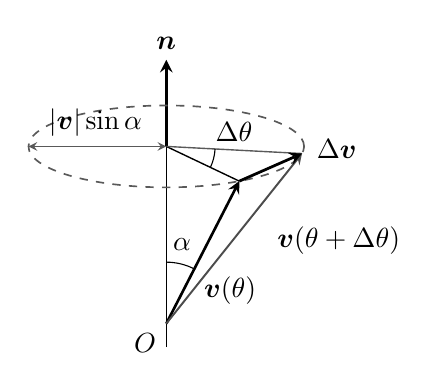
\begin{tikzpicture}[>=stealth, thick, scale=1.0]
  % Origin O at (0,0), rotation axis n along vertical
  \coordinate (O) at (0, 0);
  \coordinate (C) at (0, 2.25);

  % Rotation axis n
  \draw[line width=0.5pt] (0, -0.3) -- (0, 3.25);
  \draw[->, line width=1.0pt] (0, 2.25) -- (0, 3.35) node[above] {$\boldsymbol{n}$};
  \node[below left] at (O) {$O$};

  % Horizontal circle of rotation (ellipse in perspective) centered at C=(0,2.25)
  \draw[dashed, line width=0.6pt, black!65] (C) ellipse (1.75 and 0.52);

  % Point P = v(theta) at angle -58 deg on ellipse
  \coordinate (P) at ({1.75*cos(-58)}, {2.25 + 0.52*sin(-58)});
  % Point Q = v(theta + Delta theta) at angle -10 deg on ellipse
  \coordinate (Q) at ({1.75*cos(-10)}, {2.25 + 0.52*sin(-10)});

  % Vectors v(theta) and v(theta + Delta theta)
  \draw[->, line width=0.95pt] (O) -- (P);
  \node[below right] at (0.35, 0.72) {$\boldsymbol{v}(\theta)$};
  \draw[->, line width=0.7pt, black!70] (O) -- (Q);
  \node[right] at (1.28, 1.05) {$\boldsymbol{v}(\theta + \Delta\theta)$};

  % Radius lines from C to P and Q
  \draw[line width=0.5pt] (C) -- (P);
  \draw[line width=0.5pt, black!65] (C) -- (Q);

  % Radius length label on left horizontal radius (cleanly away from right sector)
  \draw[<->, line width=0.4pt, black!65] (-1.75, 2.25) -- (C);
  \node[above] at (-0.90, 2.25) {$|\boldsymbol{v}|\sin\alpha$};

  % Displacement arrow P -> Q
  \draw[->, line width=1.0pt] (P) -- (Q);
  \node[right] at (1.78, 2.22) {$\Delta\boldsymbol{v}$};

  % Angle alpha between n and v(theta)
  \draw[line width=0.4pt] (0, 0.78) arc (90:62.5:0.78);
  \node[above] at (0.20, 0.80) {$\alpha$};

  % Angle Delta theta between CP and CQ
  \draw[line width=0.4pt] ({0.62*cos(-25)}, {2.25 + 0.62*sin(-25)}) arc (-25:-3:0.62);
  \node[above] at (0.86, 2.18) {$\Delta\theta$};
\end{tikzpicture}
\end{document}
